\documentclass[xcolor=pdftex,dvipsnames]{beamer}

\usepackage{amsmath}
\usepackage{amssymb}

\usepackage{comment}
\usepackage{textcomp}

\title{Microeconomic Theory --- ECON 323 503 \\ Chapter 7: Costs}
\author{Vikram Manjunath}
\institute{Texas A\&M University}
\setbeamertemplate{navigation symbols}{}
\setbeamertemplate{footline}{}
\usefonttheme{serif}
\begin{document}

\maketitle

\begin{frame}
\frametitle{Outline}
\begin{enumerate}[<+->]
\item Measuring costs: must account for both explicit and
  \emph{implicit} cots.
\item Short-run costs: minimize costs by picking the right amount of
  the variable inputs for give fixed inputs.
\item Long-run costs: minimize cots by choosing the right amount of
  every input.
\item Lower costs in the long-run: more flexibility means lower costs.
\item Cost of producing multiple goods.
\end{enumerate}
\end{frame}

\begin{frame}
\frametitle{Measuring costs}
\begin{itemize}[<+->]
\item Explicit costs: wages paid for labor, price of raw material,
  etc.
\item Implicit costs: the opportunities  foregone when using resources.
\end{itemize}

\end{frame}



\begin{frame}
\frametitle{Opportunity cost}
What's it cost for you to be here in this room?

\bigskip
\uncover<2->{You paid tuition. So is that all it costs you?}

\bigskip
\uncover<3->{You're also giving up opportunities do other things. }

\bigskip
\uncover<4->{The value of those other opportunities is your ``opportunity cost'' of
being here today.}
\end{frame}



\begin{frame}
\frametitle{Opportunity cost: another example}
You start a firm and own it. 
\bigskip

\uncover<2->{You get all of the profits.}
\bigskip

\uncover<3->{You pay yourself \$1,000 as a salary.}

\bigskip
\uncover<4->{However, you could make \$11,000 working for another firm.}

\bigskip
\uncover<5->{Your opportunity cost of working for yourself is \$11,000.}

\bigskip
\uncover<6->{That's the value that you'd get from the \emph{best alternative use of
  your time}.}

\bigskip
\uncover<7->{So your cost of employing yourself isn't the \$1,000 you pay yourself,
but the \$11,000 you're forgoing. }


\end{frame}



\begin{frame}
\frametitle{Capital costs}

Decisions made apply to certain timeframes. So costs need to be
measured over those timeframes. 
\bigskip

\uncover<2->{
Two problems in measuring the cost of durable goods (capital).
}

\begin{enumerate}\uncover<3->{\item How do you spread the cost over time?}
\uncover<4->{\item How do you deal with changes in the value of capital?}
\end{enumerate}
\end{frame}



\begin{frame}
\frametitle{Capital costs: an example}
A pick-up truck costs your firm \$20,000 to buy and \$400 a month to
rent.

\bigskip
\uncover<2->{What is the monthly cost of using this pickup truck?}

\bigskip
\uncover<3->{If you rent it: \$400. If the rental rate changes over time, that's
fine too. The opportunity cost of the truck is just what you pay to
rent it.}

\bigskip
\uncover<4->{If you buy it: This is a bit more complicated.}
\bigskip

\uncover<5->{You could consider it a \$20,000 cost for the first month but is it
free afterwards?}
\bigskip

\uncover<6->{No. There's an opportunity cost: you could rent out the truck or even
sell it rather than using it.}


\end{frame}



\begin{frame}
\frametitle{Capital costs: an example}
Suppose you sell it after the first year for \$17,000. 
\bigskip

\uncover<2->{What was your opportunity cost of the truck? 
Is it \$20,000 - \$17,000 = \$3,000?}

\bigskip
\uncover<3->{No, you have to think about what you could have done with the money if
you hadn't paid for the truck. If your bank gives you (5\%) interest,
you'd have gotten back \$21,000 if you
 just deposited the money.}
\bigskip

\uncover<4->{That \$1,000 is part of the opportunity cost of the truck, bringing
its total opportunity cost to \$4,000.}
\end{frame}



\begin{frame}
\frametitle{Capital costs: another example}
If you're running a business in a building that you own, is your cost
for office space zero?

\bigskip
\uncover<2->{No. You have to account for what others might have paid you for the
space if you rented it to them rather than using it yourself. }

\bigskip
\uncover<3->{You're forgoing that additional income from the resources that you
have. That's an opportunity cost.}
\end{frame}



\begin{frame}
\frametitle{Sunk costs}
\emph{A past expenditure that cannot be recovered.}

\bigskip
\uncover<2->{These \underline{must not} be considered in making decisions.}

\bigskip
\uncover<3->{An example: expenditure on specialized/custom equipment that you can't
sell to anyone.}
\end{frame}



\begin{frame}
\frametitle{Sunk costs: an example}
You buy a piece of land for \$300,000.

\bigskip
\uncover<2->{It's market value now falls to \$200,000.}


\bigskip
\uncover<3->{The money that you lost on the land  is a \emph{sunk cost} ($\$300,000-\$200,000 = \$100,000$).}

\bigskip
\uncover<4->{You can choose to build a factory on it. With the factory on it, the
land is worth \$240,000 to you. Should you build the factory?}

\bigskip
\uncover<5->{Yes. By building the factory you end up with something worth \$40,000
$=\$240,000 - \$200,000$ more.}

\bigskip
\uncover<6->{If you considered the original cost (which you've already paid), you'd
come to the conclusion that if you build the factory, you'd have a
loss of \$60,000.}
\end{frame}



\begin{frame}
\frametitle{Short-run costs}
If you rent a space for your business, you have to pay that amount
every month. You could decide not to do any business at all and avoid
it (so it's not a sunk cost), but if you do any business at all you
have to pay rent. This is your \emph{fixed cost, F}. How much business
you do doesn't affect it.
\bigskip

\uncover<2->{The cost of inputs that you can use in varying quantities (labor and
material) depending on your output is your \emph{variable cost, VC(q)}.}
\bigskip

\uncover<3->{Your \emph{cost, C(q)} is the sum of these two:
\[
C(q) = VC(q)+F.
\]}

\end{frame}





\begin{frame}
\frametitle{Marginal cost}
If you're producing $q$ units already, what's the extra cost of
producing one more unit?
\[
\text{\emph{Marginal cost}}= MC(q) = \frac{dC(q)}{dq}.
\]

\uncover<2->{Since $F$ is a constant, $MC(q) = \frac{VC(q)}{dq}$.}

\end{frame}



\begin{frame}
\frametitle{Average cost}
\begin{enumerate}[<+->]
\item Average Fixed Cost: $AFC(q)=\frac{F}{q}$. This shrinks as $q$ grows
  large.
\item Average Variable Cost: $AVC(q) =\frac{VC(q)}{q}$. Since $VC(q)$ may
  rise or fall with $q$, this $AVC(Q)$ may rise or fall as well.
\item Average Cost: $AC(a)=\frac{C(q)}{q}$.
\[
AC(q) = \frac{C(q)}{q} = \frac{VC(q)}{q} + \frac{F}{q} = AVC(q)+AFC(q).
\]
\uncover<4->{$AC(q)$ is what you need to know if you're making a profit or not.}
\end{enumerate}
\end{frame}



\begin{frame}
\frametitle{Solved problem 7.2}
\[
C(q) = 100q - 4q^2 + 0.2q^3 + 450
\]

What are $F$ and $VC(q)$?
\uncover<2->{
\[F=450\]
}

\uncover<3->{\[VC(q) = 100q - 4q^2 + 0.2q^3\]}
\end{frame}

\begin{frame}
\frametitle{Solved problem 7.2}
Marginal cost?


\[\begin{array}{rcl}MC(q)& =& \frac{dC(q)}{dq}\\\\
&=& \frac{d(100q - 4q^2 + 0.2q^3 + 450)}{dq}\\\\
&=& 100 - 8q + 0.6q^2
\end{array}\]

\uncover<2->{ Average variable cost?
\[
\begin{array}{rcl}AVC(q)& =& \frac{VC(q)}{q}\\\\
&=& \frac{100q - 4q^2 + 0.2q^3}{q}\\\\
&=& 100 - 4q + 0.2q^2
\end{array}
\]}
\end{frame}

\begin{frame}
\frametitle{Solved problem 7.2}
Average fixed cost?
\[
AFC(q) = \frac{450}{q}
\]

\uncover<2->{ Average cost?
\[
\begin{array}{rcl}AC(q)& =& \frac{C(q)}{q}\\\\
&=& \frac{100q - 4q^2 + 0.2q^3+450}{q}\\\\
&=& 100 - 4q + 0.2q^2+\frac{450}{q}\\\\
&=& AVC(q) + AFC(q).
\end{array}
\]

}
\end{frame}


\begin{frame}
\frametitle{Short-run cost curves}
\begin{center}
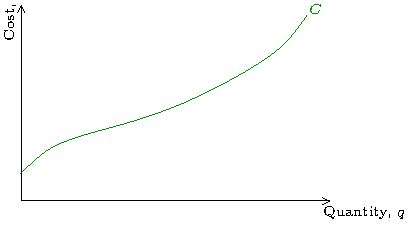
\includegraphics{pics/ShortRunCC1}
\end{center}
\ \\
\
\end{frame}

\begin{frame}
\frametitle{Short-run cost curves}
\begin{center}
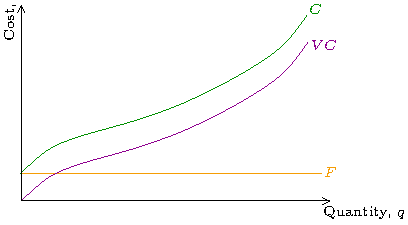
\includegraphics{pics/ShortRunCC2}
\end{center}
F doesn't vary with quantity while  VC is a curve  parallel to C (the
vertical distance between points on VC and C) is F.
\end{frame}



\begin{frame}
\frametitle{Short-run cost curves}
\begin{center}
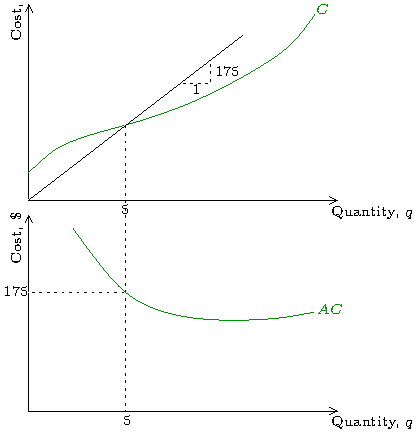
\includegraphics{pics/ShortRunCC3}
\end{center}
Average cost  is the slope of a line from 0 to a point on C.
\end{frame}



\begin{frame}
\frametitle{Short-run cost curves}
\begin{center}
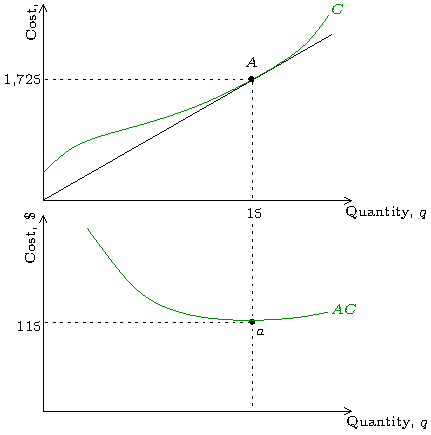
\includegraphics{pics/ShortRunCC4}
\end{center}
Average cost is minimized at $q=15$.
\end{frame}

\begin{frame}
\frametitle{Short-run cost curves}
\begin{center}
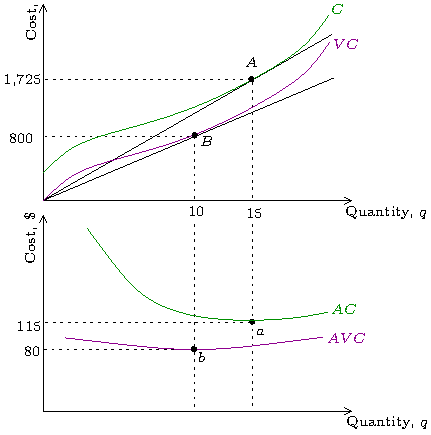
\includegraphics{pics/ShortRunCC5}
\end{center}
Similarly, AVC is minimized at $q=10$.
\end{frame}

\begin{frame}
\frametitle{Short-run cost curves}
\begin{center}
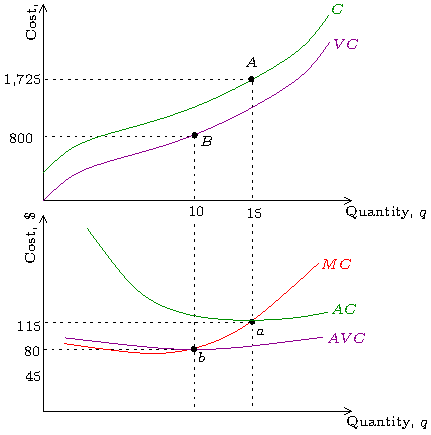
\includegraphics{pics/ShortRunCC6}
\end{center}
At each $q$, both C and VC have the same slope = MC.
\end{frame}

\begin{frame}
\frametitle{Short-run cost curves}
\begin{center}
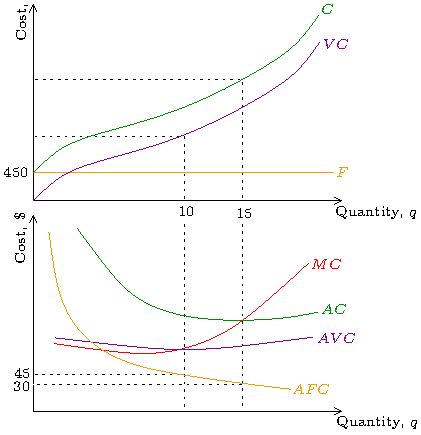
\includegraphics{pics/ShortRunCC7}
\end{center}
AFC is decreasing in $q$.
\end{frame}


\begin{frame}
\frametitle{Production functions and the shape of cost curves}
Production functions + prices of inputs  $\longrightarrow$ cost curves

\bigskip

\uncover<2->{ If your only variable cost is labor and you use $L$ units of it to
produce $q$ units of output, $VC(q) = wL$ where $w$ is the wage.}

\bigskip

\uncover<3->{ Suppose that $q=f(L,\overline K) = g(L)$. }
\bigskip

\uncover<4->{ So $L$ units of input gives us $g(L)$ units of output.}

\bigskip
\uncover<5->{ It takes $g^{-1}(q)$ units of input to produce $q$ units of output. }

\bigskip
\uncover<6->{ So $VC(q) = wg^{-1}(q)$.}
\bigskip

\uncover<7->{ Derive MC and AVC from $g$.}




\end{frame}




\begin{frame}
\frametitle{Shape of MC curve}
\[
MC(q)=\frac{dVC(q)}{dq}=\frac{dwg^{-1}(q)}{dq} = w\dfrac{1}{\frac{dg}{dq}}
= w\frac{1}{MP_L}.
\]\bigskip

\uncover<2->{
\begin{tabular}{rcl}
Diminishing $MP_L$&$\Rightarrow$ &$MP_L$ eventually decreases\\&
$\Rightarrow$&$MC$ eventually increases.
\end{tabular}
}


\end{frame}




\begin{frame}
\frametitle{Shape of AC curve}
\[
AC(q)=\frac{VC(q)}{q} = \frac{wg^{-1}(q)}{q} =
\dfrac{w}{\frac{q}{g^{-1}(q)}}= \dfrac{w}{\frac{q}{L}}= \frac{1}{AP_L}
\]

\bigskip
\uncover<2->{ We saw that $AP_L$ rises the falls so $AC$ falls then rises.}
\end{frame}




\begin{frame}
\frametitle{Effects of taxes on costs}
Specific tax of \$10 affects variable cost, but not fixed cost.
\medskip

\uncover<2->{ So AFC remains the same while AVC is shifted upwards by \$10.}
\medskip

\uncover<3->{ Similarly, MC is shifted upwards by \$10.}

\uncover<4->{
\begin{center}
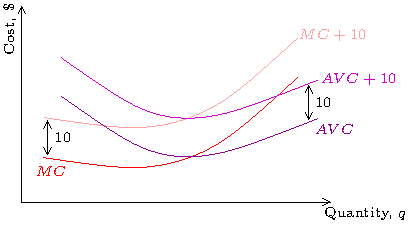
\includegraphics{pics/Tax}
\end{center}}
\end{frame}




\begin{frame}
\frametitle{Long run costs}
Recall: all inputs can be varied.
\bigskip

\uncover<2->{ Assume $F=0$ since all inputs can be varied. (Really, some
inputs are ``avoidable'' fixed costs, like rent: you can stop renting a business if
you choose not to operate).}

\bigskip
\uncover<3->{ So \[
C(q) =VC(q)
\]}

\uncover<4->{ Long run cost is never higher than short run costs. Why?}

\bigskip
\uncover<5->{ In the long run, you'd never be stuck with the wrong amount of inputs
that are fixed in the short run. You've got more flexibility.
}
\end{frame}




\begin{frame}
\frametitle{Input choice}
Recall: An isoquant is a curve through all combinations of inputs that
can be used to efficiently produce a particular amount of output.


\bigskip
\uncover<2->{\emph{Isocost} lines are all of the pairs of inputs that cost the
same.}

\bigskip
\uncover<3->{ Somewhat like a budget line.}
\end{frame}




\begin{frame}
\frametitle{Isocost line}
$w$ --- wage\\
$r$ --- rental rate
\bigskip

\uncover<2->{ All pairs $(L,K)$ that cost $\overline C$:\[
\overline C=wL+rK
\]}

\uncover<3->{ To plot this, you can re-write it as 
\[
K=\frac{\overline C}{r} - \frac{w}{r}L.
\]}
\uncover<4->{ Slope is $-\frac{w}{r}$ and vertical intercept is ${\overline C}{r}$
and horizontal intercept is ${\overline C}{w}$.}
\end{frame}




\begin{frame}
\frametitle{Isocost line}
$w=\$5$ and $r=\$8$.
\begin{center}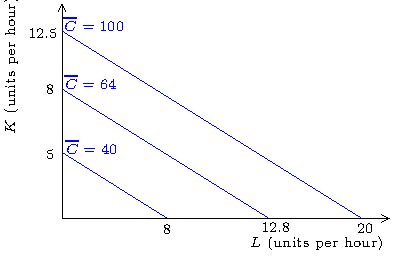
\includegraphics{pics/IsoCost}\end{center}
Higher isocost lines correspond to higher costs.
\end{frame}




\begin{frame}
\frametitle{Minimizing cost}
What is the cheapest way to produce a given level of output?

\bigskip
\uncover<2->{Three ways to find out:}
\begin{enumerate}
\uncover<3->{
\item Lowest-isocost rule: pick inputs where the lowest isocost line
  touches the isoquant.
}
\uncover<4->{
\item Tangency rule: pick inputs where an isoquant is tangent to
  the isoquant.
}
\uncover<5->{
\item Last-dollar rule: The last dollar spent one input should give
  you as much extra output as the last dollar spend on any other input.
}
\end{enumerate}
\uncover<6->{All equivalent.}
\end{frame}




\begin{frame}
\frametitle{Lowest-isocost rule}
\begin{center}
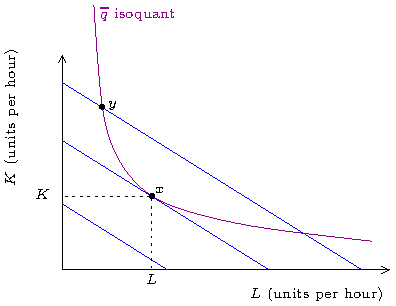
\includegraphics{pics/CostMin}
\end{center}
But this implies tangency of isocost line and isoquant.
\end{frame}




\begin{frame}
\frametitle{Tangency rule}
Recall: slope of isoquant is $MRTS$.
\bigskip

\uncover<2->{ Slope of isocost line is $-\frac{w}{r}$.}
\bigskip

\uncover<3->{ So 
\[
MRTS=-\frac{w}{r}.
\]}

\uncover<4->{ Or
\[
\frac{MP_L}{MP_K} = \frac{w}{r}.
\]}

\uncover<5->{ Rearranging this:
\[
\frac{MP_L}{w} = \frac{MP_K}{r}.
\]}
\uncover<6->{ That's the last-dollar rule.}
\end{frame}


\begin{frame} 
\frametitle{Example}
Production function:\[
q=1.52L^{0.6}K^{0.4}
\]
What is the lowest cost of producing 100 units if $w=\$24$ and $r=\$8$?

\uncover<2->{
\bigskip
Tangency rule says 
``slope of isoquant = slope of isocost.''
}

\uncover<3->{\[
MRTS=-\frac{w}{r}.
\]}
\end{frame}

\begin{frame}
\frametitle{First calculate MRTS}
\[
MRTS=-\frac{MP_L}{MP_K}.
\]

\uncover<2->{\[
MP_L = 0.6(1.52L^{-0.4}K^{0.4}) = 0.6(1.52L^{0.6}K^{0.4})L^{-1} =\frac{0.6q}{L}.
\]
}
\uncover<3->{
\[
MP_K = 0.4(1.52L^{0.6}K^{-0.6}) = 0.4(1.52L^{0.6}K^{0.4})K^{-1} =\frac{0.4q}{K}.
\]}
\uncover<4->{
\[
MRTS=-\frac{MP_L}{MP_K} = -\dfrac{\frac{0.6q}{L}}{\frac{0.4q}{K}} =
-\frac{0.6K}{0.4L} = -1.5\frac{K}{L}.
\]}


\end{frame}

\begin{frame}
\frametitle{Now set $MRTS=-\frac{w}{r}$}

\[
-1.5\frac{K}{L}=-\frac{24}{8}=-3
\]
\uncover<2->{
\[
\frac{K}{L} = \frac{3}{1.5} = 2.
\]}
\uncover<3->{
\[
K = 2L.
\]}
\uncover<4->{
Need one more equation to solve for $K$ and $L$!
}
\end{frame}


\begin{frame}
\frametitle{Production function and quantity}

You started wanting to produce 100 units:
\[
1.52 L^{0.6}K^{0.4} = 100.
\]
\uncover<2->{
Since $K=2L$,
\[
1.52L^{0.6} (2L)^{0.4} = 100
\]}
\uncover<3->{
\[1.52\times 2^{0.4} L = 100
\]
}
\uncover<4->{
\[
L = \frac{100}{1.52\times 2^{0.4}} \approx 50
\]}
\uncover<5->{ So $K=2L = 100$.}
\bigskip

\uncover<6->{ Cost of producing 100 units is:
\[wL + rK = 50 \times \$24 + 100 \times\$ 8 = \$2,000.
\]}

\end{frame}


\begin{frame}
\frametitle{Factor price changes}

Suppose that $w = \$24 \to w'=\$8$. 
\bigskip

\uncover<2->{
Isocost  slope: $-\frac{w}{r} =-\frac{24}{8}=-3\to -\frac{w'}{r}
=-\frac{8}{8}=-1$.
}
\bigskip

\uncover<3->{ New optimal way to produce 100 units is $L=77$ and $K=52$.

(This comes from setting $MRTS=-1.5\frac{K}{L} = -1$ so that $K=\frac{2}{3}L$.)}
\bigskip

\uncover<4->{ New cost of producing 100 units is \$1,032.}
\bigskip

\uncover<5->{ Notice that the firm substituted labor for capital as it became relatively cheaper. }\end{frame}


\begin{frame}
\frametitle{Is this generally true?}
Does a firm typically use more of an input as it becomes relatively
cheaper?
\bigskip

\uncover<2->{ Yes. Recall the tangency rule: $\frac{w}{r} = \frac{MP_L}{MP_K}$.}
\bigskip

\uncover<3->{ In our example: $\frac{MP_L}{MP_K} = 1.5\frac{K}{L}$. }
\bigskip

\uncover<4->{ While minimizing costs: $1.5\frac{K}{L} = \frac{w}{r}$ or $\frac{K}{L}
= w\frac{1}{1.5r}$.}
\bigskip

\uncover<5->{ Differentiating both sides with respect to $w$, 
\[
\dfrac{d\left(\frac{K}{L}\right)}{dw} = \frac{1}{1.5r}>0.
\]}
\uncover<6->{ So, holding $r$ fixed, small increases in $w$ lead to an increase of
the capital-labor ratio $\left(\frac{K}{L}\right)$.}

\end{frame}



\begin{frame}
\frametitle{How long-run cost varies with output}
\emph{Expansion path:} curve through the cost minimizing inputs for
different levels of output.

\bigskip
\uncover<2->{Back to our example with $q=1.52L^{0.6}K^{0.4}$, $w=\$24$, and
$r=\$8$.}

\bigskip
\uncover<3->{Cost of producing 100 units$= \$2,000$.}

\bigskip
\uncover<4->{Cost of producing 200 units $=\$4,000$.}

\bigskip
\uncover<5->{And so on.}
\end{frame}

\begin{frame}
\frametitle{Expansion path}
\begin{center}
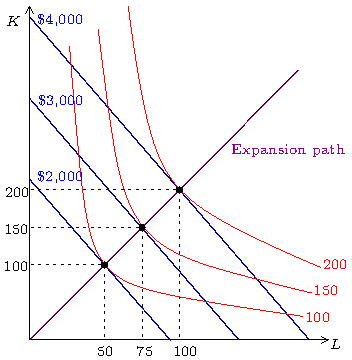
\includegraphics{pics/Expansion}
\end{center}
\end{frame}

\begin{frame}
\frametitle{Cost curve}
What does it cost to produce $q$ units?

\uncover<2->{\bigskip
Remember, that at these prices, $K=q=2L$.}

\bigskip
\uncover<3->{So
\[
C(q) = wL + rK = w\frac{q}{2} + rq = \left(\frac{w}{2} +r\right) q =
\left(\frac{24}{2} + 8\right)q = 20q.
\]}
\end{frame}




\begin{frame}
\frametitle{Cost curve}
\begin{center}
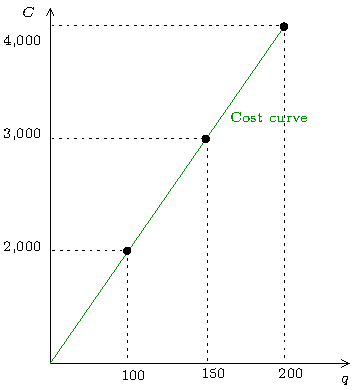
\includegraphics{pics/Cost}
\end{center}
\end{frame}




\begin{frame}
\frametitle{Cost curve}
A word of caution:

\bigskip
\uncover<2->{The production function that we just saw was easy. }

\bigskip
\uncover<3->{Why? }
\bigskip

\uncover<4->{Because it is ``homogenous of degree one'': For each $x$,
\[
q = xf(L,K) = f(xL,xK).
\]}

\uncover<5->{It's still easy as long as the production function is ``homogenous of
degree $\gamma$'' for some $\gamma$:
\[
q = x^\gamma f(L,K) = f(xL,xK).
\]}
\uncover<6->{This means that it has the same ``returns to scale'' for all levels of output.}
\end{frame}




\begin{frame}
\frametitle{The shape of long-run cost curves}
Just like short-run: 

\begin{itemize}[<+->]\item MC and AC both depend on C.
\item If AC is U-shaped, MC cuts it at the minimum.
\end{itemize}
\bigskip

\uncover<3->{Short-run: AC is U-shaped due to fixed costs and diminishing
marginal returns.}
\bigskip

\uncover<4->{Long-run: No fixed cost and no diminishing marginal return (since all
inputs can be varied). AC shape is mostly dependent on returns to
scale.}

\bigskip
\uncover<5->{If returns to scale are increasing at first and then decreasing as
quantity increases, AC is U-shaped.}


\end{frame}




\begin{frame}
\frametitle{Scale}

For a U-shaped AC:
\begin{enumerate}
[<+->]
\item low levels of output where AC is decreasing: \emph{economies of
    scale}.
\item intermediate levels of output where AC is flat: \emph{no economies of
    scale}.
\item high levels of output where AC is increasing: \emph{diseconomies of
    scale}.
\end{enumerate}
\bigskip

\uncover<4->{Competitive industries: firms have U-shaped AC curves.}

\bigskip
\uncover<5->{Non-competitive industries: firms have either U or L-shaped AC curves.}
\end{frame}




\begin{frame}
\frametitle{Lower costs in the long run}
You can vary your capital usage effectively only in the long run. 
\bigskip

\uncover<2->{Suppose there are three different plant sizes you can choose from:
small, medium, and large.}
\bigskip

\uncover<3->{Suppose the three short-run average costs of producing $q$ units are:
$SRAC^s(q), SRAC^m(q)$, and $SRAC^l(q)$.}

\bigskip
\uncover<4->{If you can simultaneously pick labor \emph{and} capital, what is the
(long-run) cost of producing $q$ units? }
\uncover<5->{\[
LRAC(q) = \min\{SRAC^s(q), SRAC^m(q), SRAC^l(q)\}.
\]}
\end{frame}




\begin{frame}
\frametitle{Lower costs in the long run}
\begin{center}
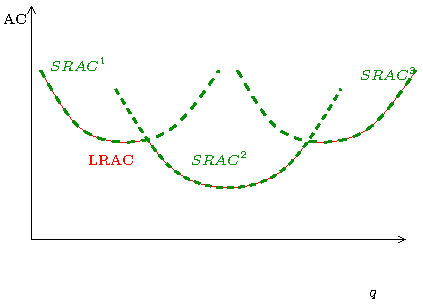
\includegraphics{pics/LRAC}
 \end{center}
Long-run AC is the least of the short-run ACs.
\end{frame}

\begin{frame}
\frametitle{Lower costs in the long run}
\begin{center}
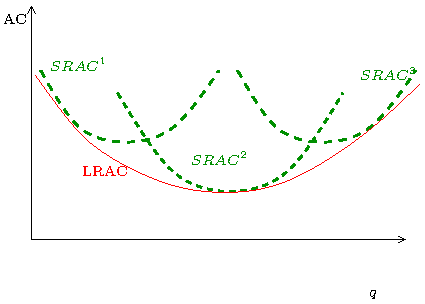
\includegraphics{pics/SmoothLRAC}
 \end{center}
If the choice of K isn't only whole numbers, LRAC is smooth.
\end{frame}




\begin{frame}
\frametitle{Example}

Laser printer:  \$$100+4$\textcent\ per page.

\bigskip
\uncover<2->{Inkjet printer:  \$$30+7$\textcent\ per page.}

\bigskip
\uncover<3->{Cost functions:
\[\begin{array}{rcl}
AC^{\text{Laser}}(q)& =& \frac{100}{q} + 0.04\\\\
AC^{\text{Inkjet}}(q)& =& \frac{30}{q} + 0.07
\end{array}
\]}


\uncover<4->{Which one should you buy?}

\uncover<5->{ It depends on $q$:
\[
LRAC(q) = \left\{\begin{array}{l}
\frac{100}{q} + 0.04 \text{ if }q>2,333\\\\
\frac{30}{q} + 0.07 \text{ if }q\leq 2,333
\end{array}\right.
\]}
\end{frame}




\begin{frame}
\frametitle{Example}
\begin{center}
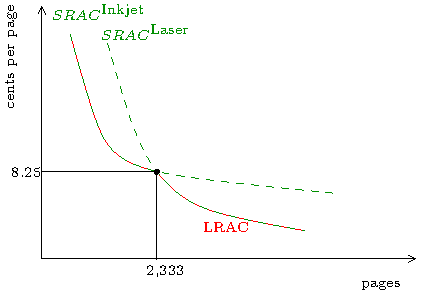
\includegraphics{pics/Printer}
 \end{center}

\end{frame}




\begin{frame}
\frametitle{Constant returns to scale and long-run AC/MC}
\begin{center}
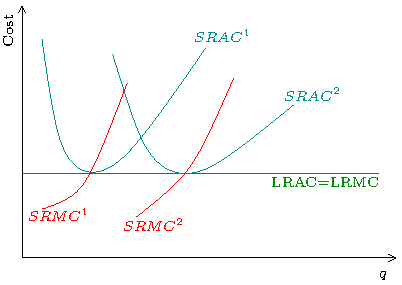
\includegraphics{pics/CRSLRAC}
 \end{center}

$CRS\Rightarrow MC=AC$ in the long run. 
\end{frame}




\begin{frame}
\frametitle{Short-run and long-run expansion paths}
\begin{center}
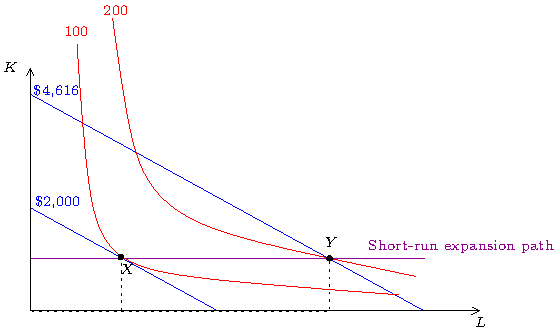
\includegraphics{pics/SRLRExpansionA}
 \end{center}
 Short-run expansion path: horizontal line at fixed $K$.
\end{frame}


\begin{frame}
\frametitle{Short-run and long-run expansion paths}
\begin{center}
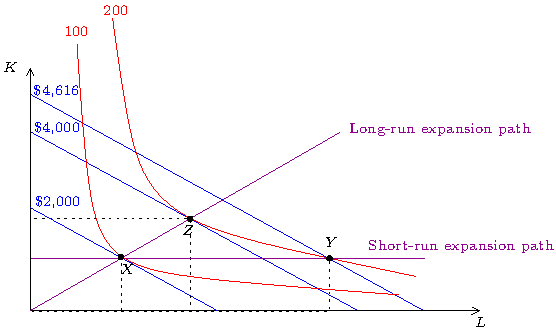
\includegraphics{pics/SRLRExpansion}
 \end{center}

Long-run expansion path: both inputs are varied.
\end{frame}




\begin{frame}
\frametitle{Learning by doing}
Reasons for long-run costs being lower than short-run costs:
\begin{enumerate}[<+->]
\item More flexibility in choosing inputs.
\item Technological progress.
\item Learning by doing: the more your output (cumulatively), the more efficiently
  you produce it.
\end{enumerate}

\end{frame}




\begin{frame}
\frametitle{Learning by doing}
\begin{center}
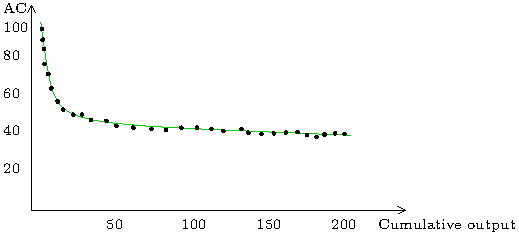
\includegraphics{pics/LBD1}
 \end{center}
Learning curve.
\bigskip

\uncover<2->{Despite common usage, a ``steep learning curve'' means you make quick progress!}
\end{frame}




\begin{frame}
\frametitle{Learning by doing: average cost over time}
\begin{center}
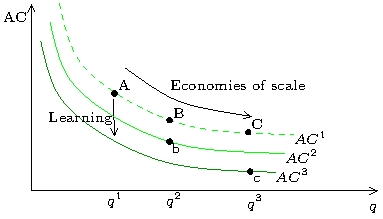
\includegraphics{pics/LBD2}
 \end{center}
Larger output means:

\uncover<2->{
 1. lower average cost today because of economies
of scale.}

\uncover<3->{
2.  lower average cost tomorrow because of learning by doing.}
\end{frame}



\begin{frame}
\frametitle{Cost of producing multiple goods}

\emph{Economies of scope:} It's less expensive to produce goods
together than it is separately.

\bigskip
\uncover<2->{Measure of ``scope'':
\[
SC = \frac{C(q_1,0)+C(0,q_2) - C(q_1,q_2)}{C(q_1,q_2)}.
\]}


\uncover<3->{$C(q_1,0)$ --- Cost of producing only good 1.\medskip}

\uncover<4->{$C(0,q_2)$ --- Cost of producing only good 2. \medskip}

\uncover<5->{$C(q_1,q_2)$ --- Cost of producing both goods together. \medskip}

\uncover<6->{$C(q_1,0)+ C(0,q_2) - C(q_1,q_2)$ --- Saving from joint production.\medskip}




\end{frame}





\begin{frame}
\frametitle{Economies of scope}
If $SC=0$ then $C(q_1,0)+ C(0,q_2) = C(q_1,q_2)$: producing the goods
separately costs the same as producing them together.
\bigskip

\uncover<2->{If $SC<0$ then $C(q_1,0)+ C(0,q_2) <  C(q_1,q_2)$: producing the goods
separately costs \emph{more} than producing them together. 
\emph{Diseconomies of scope}.\bigskip}

\uncover<3->{If $SC>0$ then $C(q_1,0)+ C(0,q_2) >  C(q_1,q_2)$: producing the goods
separately costs \emph{less} than producing them
together. \emph{Economies of scope}.}


\bigskip


\end{frame}





\begin{frame}
\frametitle{Production possibility frontier}
\begin{center}
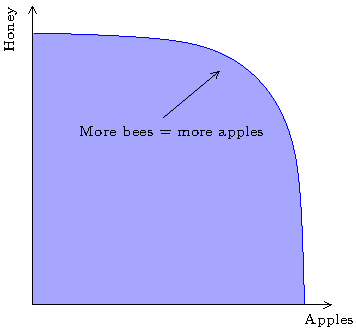
\includegraphics{pics/PPF1}
\end{center}
Production possibility set is all of the pairs of output a fixed
amount of input yields.
\bigskip

Production possibility \emph{frontier} is the boundary of this set.
\end{frame}

\begin{frame}
\frametitle{Production possibility frontier}
\begin{center}
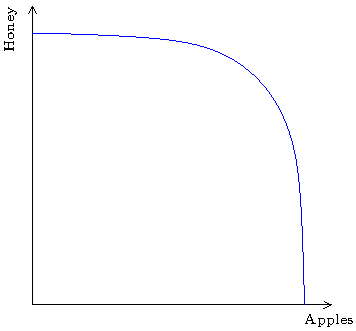
\includegraphics{pics/PPF2}
\end{center}


Economies of scope: $PPF$ bowed outwards (from origin). 
\end{frame}


\begin{frame}
\frametitle{Production possibility frontier}
\begin{center}
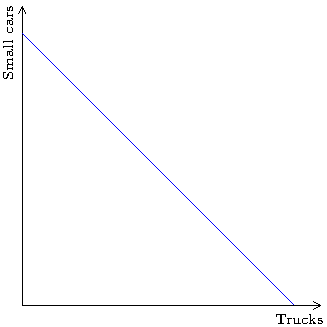
\includegraphics{pics/PPF3}
\end{center}



No economies of scope: $PPF$ straight line. 
\end{frame}


\begin{frame}
\frametitle{Production possibility frontier}
\begin{center}
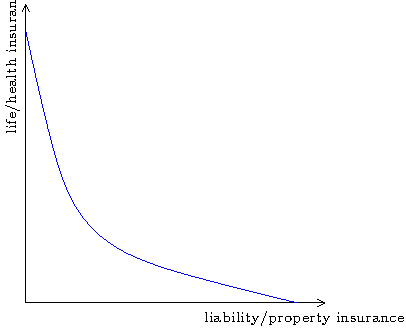
\includegraphics{pics/PPF4}
\end{center}



Diseconomies of scope: $PPF$ bowed inwards. 
\end{frame}


\end{document}






